\documentclass[11pt]{article}
\usepackage[utf8]{inputenc}\usepackage[T1]{fontenc}\usepackage{lmodern}\usepackage{microtype}
\usepackage[english]{babel}\usepackage[a4paper,margin=2.5cm]{geometry}
\usepackage{amsmath,amssymb,amsthm}\usepackage{graphicx}\usepackage{booktabs,longtable,array,calc}
\usepackage[hidelinks]{hyperref}\usepackage[capitalise,noabbrev]{cleveref}\usepackage{newunicodechar}
\newunicodechar{η}{\ensuremath{\eta}}
\newunicodechar{Δ}{\ensuremath{\Delta}}
\newunicodechar{σ}{\ensuremath{\sigma}}
\newunicodechar{μ}{\ensuremath{\mu}}
\newunicodechar{≥}{\ensuremath{\geq}}
\newunicodechar{≤}{\ensuremath{\leq}}
\newunicodechar{×}{\ensuremath{\times}}
\newunicodechar{→}{\ensuremath{\to}}
\newunicodechar{≈}{\ensuremath{\approx}}
\newunicodechar{−}{\ensuremath{-}}
\newunicodechar{·}{\ensuremath{\cdot}}
\newunicodechar{∈}{\ensuremath{\in}}
\newunicodechar{…}{\ensuremath{\ldots}}
\newunicodechar{²}{\ensuremath{^{2}}}
\newunicodechar{³}{\ensuremath{^{3}}}
\newunicodechar{√}{\ensuremath{\surd}}
\newunicodechar{±}{\ensuremath{\pm}}
\newunicodechar{⁻}{\ensuremath{^{-}}}
\newunicodechar{¹}{\ensuremath{^{1}}}
\newunicodechar{₀}{\ensuremath{_{0}}}
\newunicodechar{₁}{\ensuremath{_{1}}}
\newunicodechar{₂}{\ensuremath{_{2}}}
\newunicodechar{α}{\ensuremath{\alpha}}
\newunicodechar{β}{\ensuremath{\beta}}
\newunicodechar{γ}{\ensuremath{\gamma}}
\newunicodechar{ε}{\ensuremath{\varepsilon}}
\newunicodechar{τ}{\ensuremath{\tau}}
\newunicodechar{ν}{\ensuremath{\nu}}
\newunicodechar{∞}{\ensuremath{\infty}}
\newunicodechar{≠}{\ensuremath{\neq}}
\newunicodechar{π}{\ensuremath{\pi}}
\newunicodechar{λ}{\ensuremath{\lambda}}
\newunicodechar{ρ}{\ensuremath{\rho}}
\newunicodechar{θ}{\ensuremath{\theta}}

\providecommand{\tightlist}{\setlength{\itemsep}{0pt}\setlength{\parskip}{0pt}}
\newtheorem{theorem}{Theorem}\newtheorem{proposition}[theorem]{Proposition}\newtheorem{lemma}[theorem]{Lemma}\newtheorem{corollary}[theorem]{Corollary}
\theoremstyle{definition}\newtheorem{definition}[theorem]{Definition}\newtheorem{example}[theorem]{Example}
\newtheorem{observation}[theorem]{Numerical observation}\theoremstyle{remark}\newtheorem{remark}[theorem]{Remark}
\title{Error rates below $e^{-2\Delta}$ in two-bound-state proofreading networks: exact classification of 88 topologies and certified counterexamples}
\author{Colin Ji \and Laurenz Thümmler \and Noah Schittenhelm \and Ali Suleman\\[2pt] \small ETH Zürich}
\date{Preprint, \today}
\begin{document}
\maketitle
\begin{abstract}
An enzyme discriminates a right substrate R from a wrong substrate W by kinetic proofreading. For the linear Hopfield chain with \(n\) stages, the error rate is compared with the limit \(e^{-(n+1)\Delta}\). The classification of two-bound-state networks and its counterexamples were not found in a targeted literature search. We fix \(\Delta=\ln 100\). For \(n=2\) we prove \(\eta\ge e^{-3\Delta}\) for all positive rates and fuel potentials. Among the 88 non-degenerate two-bound-state topologies, 50 provably obey \(\eta\ge e^{-2\Delta}\), three (fam2\_66, fam2\_9, fam2\_11) have exactly certified counterexamples, and 35 remain open. The topology fam2\_66 reaches \(\eta=\) 5.082802e-07 at speed \(v=\) 1.4746e-03. The method combines symbolic positivity proofs with exact rational arithmetic. The main limitation is that 35 topologies are unresolved. Moreover, the counterexamples are certified only for log-rates in \([-10,10]\).

\par\medskip\noindent\textbf{Keywords:} kinetic proofreading, error rate bound, Hopfield limit, entropy production, Markov networks, exact certification
\end{abstract}
\section{Introduction}\label{introduction}

Kinetic proofreading raises specificity beyond what free-energy differences or kinetic barriers allow when the reaction is strongly but nonspecifically driven \cite{Hopfield19744135}. The accuracy of error-correcting pathways is set by the displacement of nucleoside triphosphates from equilibrium \cite{Ehrenberg19800636}. Several checking steps reach a given accuracy with less dissipation than a single step \cite{Ehrenberg19800636}. Models with more proofreading steps have better trade-offs between speed, error and dissipation \cite{Chiuchiu2023c757}. These Pareto fronts are studied numerically \cite{Chiuchiu2023c757}. Energy-relay proofreading shows trade-off relations and scaling laws \cite{Berx20240232}. Its mixed regime shows a dynamical phase transition in the error--entropy-production trade-off \cite{Berx20240232}.

Bounds also exist at the level of general principles. A fundamental error bound is fixed by the transition-state energy differences \cite{Yu202118v2,Yu20220883}. Thermodynamic uncertainty relations constrain the precision of outputs \cite{Barato20158101}. For Hopfield's original network there are scalings in which \(\sigma\ln(\mu)/P\) is asymptotically infinite \cite{Wong201738v1}. Numerical calculations suggest that more restrictive parametric assumptions restore a bound \cite{Wong201738v1}. Discrimination that is too strong can remove the nonequilibrium advantage \cite{Banerjee20262257}, and one regime is anti-proofreading \cite{Banerjee20262257}.

\textbf{Open question.} Does \(\eta\ge e^{-(n+1)\Delta}\) hold for all rates and fuel potentials? Which of the 88 non-degenerate topologies with two bound states obey \(\eta\ge e^{-2\Delta}\), and which do not?

\textbf{Contribution.} We prove the bound for the chain with \(n=2\) by a symbolic positivity argument. We classify the 88 two-bound-state topologies into proved, refuted and open members. For three members we give exactly certified counterexamples.

\textbf{Summary of results.}
- The Hopfield-bound theorem proves \(\eta\ge e^{-3\Delta}\) for the chain with \(n=2\) for all rates and fuel potentials.
- The classification theorem sorts the 88 topologies into 50 proved, 3 refuted and 35 open.
- The theorem on 50 topologies states the proved bound.
- The counterexample theorems give exactly certified counterexamples for fam2\_66 and for fam2\_9 and fam2\_11.
- The supporting propositions and the lemma cover family generation, subfamily bounds, verifier output and the self-test.
- The examples give exactly certified attainable points for the chain with \(n=1\).

\section{Model and assumptions}\label{model-and-assumptions}

Two substrates R and W traverse the same Markov network. W leaves bound states faster by the factor \(e^{\Delta}\). The error rate is \(\eta=J_W/J_R\), the speed is \(v=J_R\), and \(\sigma\) is the entropy production per product in units of \(kT\). Every edge has a reverse edge, local detailed balance holds, and cycle affinities arise only from the fuel potential \(\mu\) per activation and \(\mu_P\) per product (modelling rules of the task). Write \(D=e^{\Delta}\) and \(G=e^{\mu}\).

Fixed parameters; every entry is taken from:

{\def\LTcaptype{none} % do not increment counter
\begin{longtable}[]{@{}
  >{\raggedright\arraybackslash}p{(\linewidth - 4\tabcolsep) * \real{0.3333}}
  >{\raggedright\arraybackslash}p{(\linewidth - 4\tabcolsep) * \real{0.3333}}
  >{\raggedright\arraybackslash}p{(\linewidth - 4\tabcolsep) * \real{0.3333}}@{}}
\toprule\noalign{}
\begin{minipage}[b]{\linewidth}\raggedright
Symbol
\end{minipage} & \begin{minipage}[b]{\linewidth}\raggedright
Value
\end{minipage} & \begin{minipage}[b]{\linewidth}\raggedright
Meaning
\end{minipage} \\
\midrule\noalign{}
\endhead
\bottomrule\noalign{}
\endlastfoot
\(\Delta\) & \(\ln 100\) (\(e^{\Delta}=100\), \(e^{-\Delta}=0.01\)) & discrimination free-energy difference in \(kT\) \\
\(L\) & \(10\) & every rate, including derived reverse rates, lies in \([e^{-10},e^{10}]\) \\
\(\mu\) & \(\ge 0\), explored in \([0,20]\) & fuel potential per fuel-driven step \\
\(\mu_P\) & \(\ge 0\), explored in \([0,20]\) & chemical potential of product formation \\
max\_states & \(10\) & unbound states plus R and W copies of bound states \\
concentrations & \(1\) & absorbed into binding rates \\
rationalisation & denominator \(\le 10^{6}\) & rounding for exact certificates \\
\(k\) & \(2\) & bound states in the enumerated family (88 non-degenerate members) \\
\end{longtable}
}

The linear chain is called hopfield\_n\(n\) with \(n\) proofreading stages. The Hopfield limit is \(e^{-(n+1)\Delta}\).

\section{Method}\label{method}

Two certificate types are used.

\begin{itemize}
\tightlist
\item
  \textbf{Certificate (a), exact reachability.} Rates are rounded to rationals with denominator at most \(10^{6}\). The error rate \(\eta\) is evaluated exactly in rational arithmetic, and the entropy production is enclosed in an interval. A statement of the form ``\(\eta\le\eta_{\max}\) is attainable'' is certified if the rational rates lie in \([e^{-10},e^{10}]\) and satisfy local detailed balance.
\item
  \textbf{Certificate (b), symbolic positivity.} The difference between \(\eta\) and the claimed bound is written as a quotient \(N/D\) of polynomials. The bound holds for all positive rates and fuel potentials if all coefficients are nonnegative. This proof is independent of the rate range.
\end{itemize}

A verifier generates the topologies, enforces the model rules, and passes a self-test with 18 of 18 cases. Its code is the trusted base. Optimiser output is only a numerical candidate until it is certified by (a). Numerical scans are labelled as numerical.

The work was carried out by an automated, verifier-gated laboratory. Every statement below was accepted only after code verification (details in Appendix A).

\section{Results}\label{results}

\subsection{Main results}\label{main-results}

\begin{theorem}[Hopfield bound for the chain with $n=2$]
For hopfield\_n2, \(\eta\ge e^{-3\Delta}\) holds for all positive rates and all fuel potentials \(\mu,\mu_P\ge0\).
\end{theorem}

\textbf{Certificate.} Symbolic positivity proof (b): \(\eta-e^{-3\Delta}=N/D\) with 1374 and 2048 terms, respectively, and all coefficients nonnegative (checked in 6.8 s). Novelty status: not found in a targeted search of 40 abstracts on 2026-10-04. Qualitatively this is a reproduction of the Hopfield bound, here with a rigorous proof.

\begin{proposition}[Family generation]
For two bound states the verifier's generator produces 92 rule-conforming topologies. Four of these are degenerate (no net production possible, \(\eta=0/0\)) and are excluded. This leaves 88 non-degenerate topologies.
\end{proposition}

\begin{theorem}[Classification of two-bound-state topologies]
Of the 88 non-degenerate topologies with two bound states, 50 satisfy a proved bound \(\eta\ge e^{-2\Delta}\) (certificate (b)). Three of them (fam2\_66, fam2\_9, fam2\_11) have an exactly certified counterexample \(\eta<e^{-2\Delta}\) (certificate (a)). The remaining 35 are open.
\end{theorem}

\textbf{Certificate.} The three theorems below on the bound for 50 topologies and on the counterexamples. Novelty status: not found in the research.

{\def\LTcaptype{none} % do not increment counter
\begin{longtable}[]{@{}lll@{}}
\toprule\noalign{}
Class & Members & Certificate \\
\midrule\noalign{}
\endhead
\bottomrule\noalign{}
\endlastfoot
bound \(\eta\ge e^{-2\Delta}\) proved & 50 & (b) \\
counterexample \(\eta<e^{-2\Delta}\) & 3 & (a) \\
open & 35 & none \\
\end{longtable}
}

\emph{Table 1.} Classification of the 88 topologies.

\begin{theorem}[The bound for 50 topologies]
For 50 topologies of the verifier-generated family with at most two bound states (one unbound state, edge catalogue of the model), \(\eta\ge 1/D^{2}\) holds for all positive rates and fuel potentials.
\end{theorem}

\textbf{Certificate.} Symbolic certificate (b): the bound is proved for 50 of 50 members. Novelty status: not found in a targeted search of 48 abstracts on 2026-10-04.

\begin{theorem}[Counterexample fam2_66]
For fam2\_66 there exist rational rates in \([e^{-10},e^{10}]\) satisfying local detailed balance with \(\eta\le 0.0001\) and \(v\ge 0.0001\). The exact values are \(\eta=\) 5.082802e-07, \(\sigma=\) 8.341626 \(kT\) per product and \(v=\) 1.4746e-03.
\end{theorem}

\textbf{Certificate.} Certificate (a), exact rational evaluation, with \(\sigma\in[8.341626,8.341626]\). The edges of fam2\_66 are binding to C0, a fuel-driven conversion C0 to C1, a fuel-driven discard from C1, and product formation from C1. Novelty status: not found in a targeted search of 48 abstracts on 2026-10-04.

\begin{theorem}[Counterexamples fam2_9 and fam2_11]
For each of the two topologies fam2\_11 and fam2\_9 there exist rational rates in \([e^{-10},e^{10}]\) satisfying local detailed balance with \(\eta\le 0.0001\).
\end{theorem}

\textbf{Certificate.} Certificate (a) passed for 2 of 2 cases. Novelty status: not found in a targeted search of 42 abstracts on 2026-10-04.

\subsection{Supporting statements}\label{supporting-statements}

\begin{proposition}[Subfamily bound]
For 3 topologies of the verifier-generated family with at most two bound states, \(\eta\ge 1/D^{2}\) holds for all positive rates and fuel potentials.
\end{proposition}

\textbf{Certificate.} Symbolic certificate (b): 3 of 3 members proved.

\begin{proposition}[Subfamily bound, second question]
The same conclusion holds for 3 topologies when the question is whether a fuel-driven discard exit at the product state is necessary.
\end{proposition}

\textbf{Certificate.} Symbolic certificate (b): 3 of 3 members proved. This verified result is subsumed by the theorem on 50 topologies, and by itself does not decide necessity of the discard exit.

\begin{lemma}[Verifier output of the counterexample round]
The verifier output of round 12 is: certificate (a) passed for 2 of 2 cases.
\end{lemma}

\begin{proposition}[Verifier self-test]
The verifier passes its self-test with 18 of 18 cases (true, false, borderline, rule-violating).
\end{proposition}

\subsection{\texorpdfstring{Examples (chain with \(n=1\))}{Examples (chain with n=1)}}\label{examples-chain-with-n1}

These are attainable points. They certify reachability, not optimality.

\begin{example}[Moderate dissipation]
For hopfield\_n1 there exist rational rates in \([e^{-10},e^{10}]\) satisfying local detailed balance with \(\eta\le 0.0004\), \(\sigma\le 6.0\) \(kT\) per product and \(v\ge 0.001\).
\end{example}

The certificate gives \(\eta=\) 3.650169e-04, \(\sigma\in[6.000000,6.000000]\) and \(v=\) 1.0417e-01. Novelty status: not found in a targeted search of 62 abstracts on 2026-10-04.

\begin{example}[Moderate error rate]
For hopfield\_n1 there exist rational rates with \(\eta\le 0.01\) and \(v\ge 0.001\).
\end{example}

The certificate gives \(\eta=\) 5.909757e-03, \(\sigma\in[3.998555,3.998555]\) and \(v=\) 7.1214e-03. Novelty status: not found in a targeted search of 45 abstracts on 2026-10-04.

\begin{example}[Very low dissipation]
For hopfield\_n1 there exist rational rates with \(\eta\le 0.00012\) and \(\sigma\le 0.2\) \(kT\) per product.
\end{example}

The certificate gives \(\eta=\) 1.095823e-04, \(\sigma\in[0.006292,0.006292]\) and \(v=\) 9.1487e-09. Novelty status: not found in a targeted search of 49 abstracts on 2026-10-04.

\begin{example}[Speed constraint]
For hopfield\_n1 there exist rational rates with \(\eta\le 0.0002\), \(\sigma\le 10\) \(kT\) per product and \(v\ge 0.001\).
\end{example}

The certificate gives \(\eta=\) 1.189200e-04, \(\sigma\in[4.271813,4.271813]\) and \(v=\) 1.0000e-03. Novelty status: not found in a targeted search of 37 abstracts on 2026-10-04. Attainable points of the chain are qualitatively known, and are here exact.

{\def\LTcaptype{none} % do not increment counter
\begin{longtable}[]{@{}lllll@{}}
\toprule\noalign{}
Case & \(\eta\) & \(\sigma\) (\(kT\)) & \(v\) & Source \\
\midrule\noalign{}
\endhead
\bottomrule\noalign{}
\endlastfoot
fam2\_66 & 5.082802e-07 & 8.341626 & 1.4746e-03 & \\
hopfield\_n1, Ex. 1 & 3.650169e-04 & 6.000000 & 1.0417e-01 & \\
hopfield\_n1, Ex. 2 & 5.909757e-03 & 3.998555 & 7.1214e-03 & \\
hopfield\_n1, Ex. 3 & 1.095823e-04 & 0.006292 & 9.1487e-09 & \\
hopfield\_n1, Ex. 4 & 1.189200e-04 & 4.271813 & 1.0000e-03 & \\
\end{longtable}
}

\emph{Table 2.} Certificate (a) data (exact rational \(\eta\), interval enclosure of \(\sigma\)).

\textbf{Remark (status of the computer-assisted parts).} The Hopfield-bound theorem and the theorem on 50 topologies rest on certificate (b). The counterexample theorems and the four examples rest on certificate (a). The trusted base is the verifier, including its exact rational arithmetic and its symbolic positivity check. A third party re-runs everything with the command in the Declarations. The optimiser that finds candidates is not trusted.

\section{Negative results}\label{negative-results}

\begin{itemize}
\tightlist
\item
  \textbf{The 35 open topologies.} For these members neither a proof of \(\eta\ge e^{-2\Delta}\) (certificate (b)) nor a certified counterexample (certificate (a)) was obtained. The reason is unknown.
\item
  \textbf{Necessity of a fuel-driven discard exit.} The question was posed in a form that asks for either a counterexample without the feature or a proof of the bound on the subfamily without it. The verified result covers only 3 topologies, so the question is not decided here. The failed attempts and their causes (verifier faults, later fixed) are documented in Appendix A.
\end{itemize}

\section{Discussion, limitations and open questions}\label{discussion-limitations-and-open-questions}

The chain with \(n=2\) respects its Hopfield limit for all rates and fuel potentials. Three two-bound-state topologies (fam2\_66, fam2\_9, fam2\_11) have certified counterexamples to \(\eta\ge e^{-2\Delta}\). The certified example fam2\_66 uses a fuel-driven discard from the product-forming state. A mixed regime with a phase transition in the front was reported in the literature \cite{Berx20240232}. A speed--accuracy trade-off need not be universal \cite{Wu20265626}. High dissipation can favour speed \cite{Yu20220883}.

\textbf{Limitations.}
- The classification is for \(\Delta=\ln 100\) and rates in \([e^{-10},e^{10}]\).
- The counterexamples are certified for rational rates with denominator at most \(10^{6}\), and for \(\mu,\mu_P\) explored in \([0,20]\).
- Counterexamples are certified at low speed. For fam2\_66, \(v=\) 1.4746e-03.
- The results concern at most \(10\) states and substrate concentrations normalised to one.
- The four examples are attainable points, not Pareto optima.

\textbf{Open questions.}
1. (i) What decides the 35 open topologies?
2. (ii) Is a fuel-driven discard exit at the product state necessary to go below \(e^{-2\Delta}\)? Only a partial result for 3 topologies exists.
3. (iii) Do bounds of the type \(e^{-(n+1)\Delta}\) hold for other chains with \(n=2\) and general branched topologies, beyond hopfield\_n2?

\section{Declarations}\label{declarations}

\textbf{AI usage.} The results were produced and checked by an automated laboratory. Every statement was verified by code.

\textbf{Code and data availability.} Repository https://github.com/alizema700/Daddys-Project, branch \texttt{claude/paper-pipeline-v2}, directory \texttt{projects/proofreading}. Reproduce all certificates with \texttt{python\ -m\ asd.recheck\ proofreading}. Rebuild the paper with \texttt{python\ -m\ asd.paper\ -\/-domain\ proofreading}.

\textbf{Competing interests.} None.

\appendix

\section{Agentic laboratory}\label{agentic-laboratory}

\textbf{Workflow.} The laboratory ran 12 rounds with 11 verified statements and 1 negative results. Every round was preregistered before the experiment.

\textbf{Roles.} The roles in the failed attempts of the negative result were sparsam, numeriker, skeptiker and theoretiker.

\textbf{Preregistration.} Preregistration H6 (commit 6184672) was made before the first run, with dated addenda. The L2c success criterion (at least 5 counterexamples in one round) was missed: 2 were found in round 12, and 3 in total.

\textbf{Literature search.} 2752 sources were retrieved (arXiv, Europe PMC, Crossref, citation chain). 2502 were screened, and 158 findings have a verbatim quote confirmed in the abstract by code. All 11 classic searches had hits.

\textbf{Red team.} In total there were 22 counter-checks, of which 4 passed, 8 did not pass and 10 were not executable.

\textbf{Negative result.} For the question on the necessity of a fuel-driven discard exit no claim passed the verifier. Four attempts (sparsam, numeriker, skeptiker, theoretiker) failed because of a verifier error that was later fixed. One boundary-case topology was rejected by the rule check: a discriminating edge is allowed only from bound to unbound.

\textbf{Additional counter-checks.}
- A counter-check of Example 1 shows that the feasible set grows with the allowed dissipation, so the minimal \(\eta\) is non-increasing. The same parameter set remains feasible at larger dissipation budgets. A reported kink in the front is therefore an optimiser artefact.
- The attempt to prove \(\eta\ge 1.2\,e^{-2\Delta}\) for the chain with \(n=1\) fails symbolically, as expected from the very-low-dissipation example.
- For fam2\_9, fam2\_11 and fam2\_13 the attempt to prove the bound gave 0 of 3 members proved. This is consistent with the certified counterexamples for fam2\_9 and fam2\_11. For fam2\_13 no counterexample is claimed here.
- An independent numerical search with 24 starts for the chain with \(n=2\) found a minimum of 3.1387e-05, which did not support a claim of a value much below \(e^{-3\Delta}\). This is numerical only, and not a proof.

\begin{example}[Supplementary: pareto-front check, appendix only]
For hopfield\_n1 there exist rational rates in \([e^{-10},e^{10}]\) satisfying local detailed balance with \(\eta\le 0.0004\), \(\sigma\le 8\) \(kT\) per product and \(v\ge 0.001\). The certificates give \(\eta=\) 3.156120e-04 at \(\sigma\in[6.000000,6.000000]\) with \(v=\) 2.4255e-02, and \(\eta=\) 2.043712e-04 at \(\sigma\in[3.079633,3.079633]\) with \(v=\) 2.2592e-03. Novelty status: not found in a targeted search of 57 abstracts on 2026-10-04.
\end{example}

\section{Provenance}\label{provenance}

The provenance table mapping every statement to its evidence follows; it is generated automatically.

{\def\LTcaptype{none} % do not increment counter
\begin{longtable}[]{@{}
  >{\raggedright\arraybackslash}p{(\linewidth - 4\tabcolsep) * \real{0.3333}}
  >{\raggedright\arraybackslash}p{(\linewidth - 4\tabcolsep) * \real{0.3333}}
  >{\raggedright\arraybackslash}p{(\linewidth - 4\tabcolsep) * \real{0.3333}}@{}}
\toprule\noalign{}
\begin{minipage}[b]{\linewidth}\raggedright
Statement
\end{minipage} & \begin{minipage}[b]{\linewidth}\raggedright
Evidence (claim ids)
\end{minipage} & \begin{minipage}[b]{\linewidth}\raggedright
Level
\end{minipage} \\
\midrule\noalign{}
\endhead
\bottomrule\noalign{}
\endlastfoot
Section: Introduction & C-fakt-familie, C-fakt-klassifikation, C-fakt-r12, C-fakt-selbsttest, C-proofreading-R1, C-proofreading-R10, C-proofreading-R11, C-proofreading-R12, C-proofreading-R3, C-proofreading-R4, C-proofreading-R6, C-proofreading-R7, C-proofreading-R8, C-proofreading-R9 & computed\_rigorous \\
Section: Model and assumptions & C-modell, C-proofreading-R3, C-proofreading-R9 & computed\_rigorous \\
Section: Method & C-fakt-selbsttest, C-modell, C-proofreading-R1, C-proofreading-R4, C-proofreading-R9 & computed\_rigorous \\
Theorem 1 (Hopfield bound for the chain with \(n=2\)) & C-proofreading-R9 & computed\_rigorous \\
Section: Main results & C-fakt-fam66, C-fakt-klassifikation, C-fakt-neuheit, C-fakt-r12, C-proofreading-R11, C-proofreading-R12, C-proofreading-R4, C-proofreading-R9 & computed\_rigorous, observed \\
Proposition 1 (Family generation) & C-fakt-familie & computed\_rigorous \\
Theorem 2 (Classification of two-bound-state topologies) & C-fakt-klassifikation & computed\_rigorous \\
Theorem 3 (The bound for 50 topologies) & C-proofreading-R11 & computed\_rigorous \\
Theorem 4 (Counterexample fam2\_66) & C-fakt-fam66, C-proofreading-R4 & computed\_rigorous \\
Theorem 5 (Counterexamples fam2\_9 and fam2\_11) & C-proofreading-R12 & computed\_rigorous \\
Proposition 2 (Subfamily bound) & C-proofreading-R6 & computed\_rigorous \\
Section: Supporting statements & C-proofreading-R11, C-proofreading-R6, C-proofreading-R7 & computed\_rigorous \\
Proposition 3 (Subfamily bound, second question) & C-proofreading-R7 & computed\_rigorous \\
Lemma 1 (Verifier output of the counterexample round) & C-fakt-r12 & computed\_rigorous \\
Proposition 4 (Verifier self-test) & C-fakt-selbsttest & computed\_rigorous \\
Example 1 (Moderate dissipation) & C-proofreading-R1 & computed\_rigorous \\
Section: Examples (chain with \(n=1\)) & C-fakt-neuheit, C-proofreading-R1, C-proofreading-R10, C-proofreading-R11, C-proofreading-R12, C-proofreading-R3, C-proofreading-R4, C-proofreading-R8, C-proofreading-R9, C-verfuegbarkeit & computed\_rigorous, observed \\
Example 2 (Moderate error rate) & C-proofreading-R3 & computed\_rigorous \\
Example 3 (Very low dissipation) & C-proofreading-R8 & computed\_rigorous \\
Example 4 (Speed constraint) & C-proofreading-R10 & computed\_rigorous \\
Section: Negative results & C-fakt-klassifikation, C-neg1, C-proofreading-R7 & computed\_rigorous, observed \\
Section: Discussion, limitations and open questions & C-fakt-fam66, C-fakt-klassifikation, C-modell, C-proofreading-R7, C-proofreading-R9 & computed\_rigorous \\
Section: Declarations & C-verfuegbarkeit & observed \\
Section: Appendix A: Agentic laboratory & C-fakt-praereg, C-fakt-recherche, C-methode, C-neg1, C-proofreading-R1-RT1, C-proofreading-R1-RT2, C-proofreading-R12, C-proofreading-R12-RT1, C-proofreading-R7-RT2, C-proofreading-R8-RT1, C-proofreading-R9-RT2, C-redteam & computed\_rigorous, observed \\
Example 5 (Supplementary: pareto-front check, appendix only) & C-proofreading-R2 & computed\_rigorous \\
Section: Appendix C: Verifier self-test & C-fakt-selbsttest, C-proofreading-R1, C-proofreading-R10, C-proofreading-R11, C-proofreading-R12, C-proofreading-R2, C-proofreading-R4, C-proofreading-R6, C-proofreading-R7, C-proofreading-R7-RT2, C-proofreading-R8, C-proofreading-R9 & computed\_rigorous, observed \\
\end{longtable}
}

The complete automatic checking protocol of the writing process is stored as pruefprotokoll.json in the project directory of the repository.

\section{Verifier self-test}\label{verifier-self-test}

The verifier of the domain passes its self-test with 18 of 18 cases, covering true statements, false statements, borderline cases and rule violations. For example, a topology that violates the model rules is rejected by the rule check.

\begin{figure}[t]\centering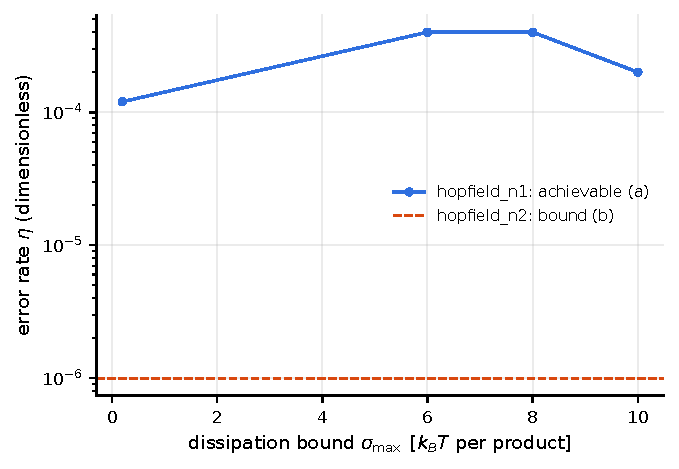
\includegraphics[width=0.75\textwidth]{pareto_front.pdf}\caption{Certified achievable error thresholds (dots; each dot is the threshold of one exact certificate, not an optimum) and proven lower bounds (dashed lines).}\end{figure}
\begin{figure}[t]\centering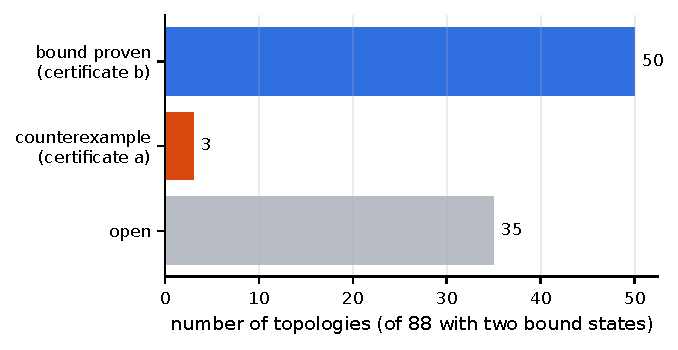
\includegraphics[width=0.75\textwidth]{klassifikation.pdf}\caption{Classification of the 88 non-degenerate networks with two bound states with respect to the bound $\eta \geq e^{-2\Delta}$.}\end{figure}

\bibliographystyle{unsrt}
\bibliography{references}
\end{document}
